\chapter{Metodi diretti per la soluzione di sistemi lineari}

\section{Introduzione}
Un \textcolor{orange}{sistema lineare} è un particolare tipo di problema diretto in cui la funzione \textcolor{orange}{$F$}
è definita come:
\[\textcolor{orange}{F(x, d) = Ax - d}\]
con $A \in \mathbb{R}^{n \times n}, x, d \in \mathbb{R}^n$.

I metodi risolutivi per i sistemi lineari sono suddivisibili
in due macro-categorie:
\begin{itemize}
\item \textcolor{orange}{Metodi diretti}: forniscono la soluzione esatta in un numero finito di operazioni.\\
Sono metodi stabili, ma hanno un costo computazionale elevato.

Esempi: eliminazione di Gauss, fattorizzazione LU, fattorizzazione Cholesky.
\item \textcolor{orange}{Metodi iterativi}:non calcola la soluzione direttamente in un unico passo, ma 
costruisce una successione di approssimazioni che si avvicinano sempre più alla soluzione esatta.\\
Sono metodi più efficienti dal punto di vista computazionale, ma possono essere instabili e non garantire la convergenza.

Esempi: metodo di Jacobi, metodo di Gauss-Seidel, metodo del gradiente coniugato.
\end{itemize}

In ogni caso però, per entrambe le categorie, non si può prescindere dagli
errori di rappresentazione e dalla loro propagazione nei calcoli.

Ad ogni modo noi ci concentreremo sullo studio dei metodi diretti.

Come ci si può aspettare, la sensibilità di un problema diretto alle perturbazioni nei dati è strettamente legata alla matrice 
$A$ che definisce il sistema lineare.

Quando in futuro cercheremo di misurare la sensibilità di un sistema lineare, ci riferiremo al seguente teorema:
\begin{theorem}[Numero di condizionamento di un sistema lineare]
    Data una \textcolor{orange}{norma  $\|\cdot\|$} su $\mathbb{R}^n$, sia \textcolor{orange}{$\|\cdot\|_m$} 
    la norma indotta su $\mathbb{R}^{n \times n}$.\\
    Si consideri un sistema lineare \textcolor{orange}{$Ax = b$} con \textcolor{orange}{$A$} invertibile.

    Il \textcolor{orange}{numero di condizionamento} del
    sistema $\textcolor{orange}{Ax = b}$ è definito come:
    \[\textcolor{orange}{K(A) = \|A\|_m \|A^{-1}\|_m}\]
\end{theorem}

\begin{proof}
    Dimostriamo che $K(A)$ è una misura della sensibilità del sistema alle perturbazioni nei dati. Consideriamo una perturbazione $\delta b$ nei dati $b$ e la corrispondente variazione $\delta x$ nella soluzione $x$. Abbiamo:
    \[
    A(x + \delta x) = b + \delta b
    \]
    Sostituendo $Ax = b$, otteniamo:
    \[
    A\delta x = \delta b
    \]
    Moltiplicando entrambi i lati per $A^{-1}$, otteniamo:
    \[
    \delta x = A^{-1} \delta b
    \]
    Prendendo le norme, otteniamo:
    \[
    \|\delta x\| \leq \|A^{-1}\|_m \|\delta b\|
    \]
    D'altra parte, abbiamo anche:
    \[
    \|b\| = \|Ax\| \leq \|A\|_m \|x\|
    \]
    Combinando queste due disuguaglianze, otteniamo:
    \[
    \frac{\|\delta x\|}{\|x\|} \leq K(A) \frac{\|\delta b\|}{\|b\|}
    \]
\end{proof}

\begin{obs}
    Per semplicità abbiamo perturbato il vettore noto $b$ ($\delta_b$), ma è possibile perturbare anche la matrice 
    $A$ ($\delta_A$) e ottenere risultati simili.
\end{obs}


Noi ci concentreremo sullo studio di sistemi definiti da matrici $A$ che sono non singolari (invertibili).

Vengono ora presentate alcune \textcolor{orange}{definizioni} di sistemi lineari e dei metodi diretti per la loro risoluzione.

\begin{defi}[Matrici diagonali]
Consideriamo un sistema lineare $Ax = b$ in cui $A$ è una matrice diagonale, ovvero:
\textcolor{orange}{\[
A = \begin{bmatrix}
a_{11} & 0 & \cdots & 0 \\
0 & a_{22} & \cdots & 0 \\
\vdots & \vdots & \ddots & \vdots \\
0 & 0 & \cdots & a_{nn}
\end{bmatrix}
\]}
In questo caso, la soluzione del sistema è immediata e data da:
\textcolor{orange}{\[
x_i = \frac{b_i}{a_{ii}} \quad \text{per } i = 1, 2, \ldots, n
\]}
\end{defi}

\begin{defi}[Matrici triangolari]
Consideriamo un sistema lineare $Ax = b$ in cui $A$ è una matrice triangolare superiore, ovvero:
\textcolor{orange}{\[
A = U = \begin{bmatrix}
a_{11} & a_{12} & \cdots & a_{1n} \\
0 & a_{22} & \cdots & a_{2n} \\
\vdots & \vdots & \ddots & \vdots \\
0 & 0 & \cdots & a_{nn}
\end{bmatrix}
\]}
In questo caso, la soluzione del sistema può essere trovata tramite il metodo di sostituzione all'indietro ($backward \, solve$), ovvero:
\textcolor{orange}{\[
x_n = \frac{b_n}{a_{nn}}, \quad x_i = \frac{b_i - \sum_{j=i+1}^n a_{ij}x_j}{a_{ii}}
\]}

Nel caso di una matrice triangolare inferiore, si utilizza invece il metodo di sostituzione in avanti ($forward \, solve$).
\textcolor{orange}{\[
A = L =\begin{bmatrix}
a_{11} & 0 & \cdots & 0 \\
a_{21} & a_{22} & \cdots & 0 \\
\vdots & \vdots & \ddots & \vdots \\
a_{n1} & a_{n2} & \cdots & a_{nn}
\end{bmatrix}
\qquad
 x_1=\frac{b_1}{a_{11}}, \quad x_i = \frac{b_i - \sum_{j=1}^{i-1} a_{ij}x_j}{a_{ii}}
\]}
\end{defi}

\begin{obs}
Nei prossimi paragrafi verranno utilizzate nuovamente le notazioni \textcolor{orange}{$U$} e \textcolor{orange}{$L$}
per indicare rispettivamente una matrice triangolare superiore (dall'inglese \textcolor{orange}{"upper triangular"}) e una matrice triangolare inferiore (dall'inglese \textcolor{orange}{"lower triangular"}).
\end{obs}

\section{Metodi diretti per la soluzione di sistemi lineari}
Molti dei metodi numerici diretti utilizzano per la risoluzione dei sistemi lineari
una \textcolor{orange}{fattorizzazione} della matrice \textcolor{orange}{$A$} nel prodotto 
di due matrici \textcolor{orange}{$B$} e \textcolor{orange}{$C$}:
\textcolor{orange}{\[A = BC\]}
La soluzione del sistema viene trovata risolvendo in successione i due sistemi lineari ausiliari:
\[
\textcolor{orange}{Ax = b \quad \Leftrightarrow \quad By = b, \, Cx = y}
\]

Fattorizzazioni diverse della matrice A sono associate a metodi risolutivi diversi. \\
Noi vedremo le seguenti fattorizzazioni:
\begin{enumerate}
\item \textcolor{orange}{Fattorizzazione LU}: \[A = LU\] dove $L$ è una matrice triangolare inferiore e $U$ è una matrice triangolare superiore.
\item \textcolor{orange}{Fattorizzazione Cholesky}: \[A = LL^T\] dove $L$ è una matrice triangolare inferiore.
 Questa fattorizzazione è applicabile solo se $A$ è simmetrica e definita positiva.
\item \textcolor{orange}{Fattorizzazione QR}: \[A = QR\] dove $Q$ è una matrice unitaria e $R$ è una matrice triangolare superiore.
\end{enumerate}

\begin{obs}
La lettera \textcolor{orange}{$R$} è spesso utilizzata per indicare una matrice triangolare superiore perchè è sinonimo in inglese
di \textcolor{orange}{$right$} (una matrice triangolare superiore è sempre una matrice quadrata e ha elementi non nulli solo nella parte destra).
\end{obs}

\subsection{Matrici elementari}

In questo paragrafo si introduce un particolare tipo di matrice, la \textcolor{orange}{matrice elementare}, che
sarà fondamentale nello studio delle fattorizzazioni.

\begin{defi}[Matrice elementare]
Siano \textcolor{orange}{$\sigma \epsilon \mathbb{R}$} e \textcolor{orange}{$u, v \in \mathbb{R}^n$} con \textcolor{orange}{$u, v \neq 0$}.
 La matrice elementare \textcolor{orange}{$E$} è definita come:
\[\textcolor{orange}{E = I - \sigma uv^T}\]
\end{defi}

La classe delle matrici elementari non singolari (ovvero invertibili) è chiusa rispetto all'operazione di inversione.\\
Vale infatti il seguente teorema.

\begin{theorem}[Inversione di una matrice elementare]\label{teorema:inversione_elementare}
    Ogni matrice elementare, \textcolor{orange}{$E(\sigma, u, v)$}, per cui valga la condizione:
    \[ 
    \textcolor{orange}{\textbf{v}^t \textbf{u} \neq \frac{1}{\sigma}}
    \]
    è \textcolor{orange}{invertibile} e la sua \textcolor{orange}{matrice inversa} è sempre una matrice elementare della forma:
    \[\textcolor{orange}{E(\tau, u, v)} \quad \text{con} \quad \textcolor{orange}{\tau \in \mathbb{R}}\]
\end{theorem}

\begin{proof}

    Se $\sigma = 0$ la tesi è ovvia, in quanto $E(0, u, v) = I$.
    
    Supponiamo ora $\sigma \neq 0$. Vogliamo dimostrare che esista $\tau \in \mathbb{R}$ tale che:
    \[
    E(\sigma, u, v) E(\tau, u, v) = I
    \]
    Sviluppando il prodotto:
    \[
    (I - \sigma uv^T)(I - \tau uv^T) = I - \sigma uv^T - \tau uv^T + \sigma \tau (uv^T)(uv^T)
    \]
    Poiché $(uv^T)(uv^T) = u(v^T u)v^T = (v^T u)uv^T$, otteniamo:
    \[
    I - (\sigma + \tau) uv^T + \sigma \tau (v^T u) uv^T
    \]
    Per ottenere l'identità, dobbiamo avere:
    \[
    -(\sigma + \tau) + \sigma \tau (v^T u) = 0
    \]
    Da cui si ottiene che $\tau$ deve soddisfare la condizione:
    \begin{equation}\label{eq.:cond_inv_elementare}
        \textbf{v}^t \textbf{u} = \frac{1}{\sigma} + \frac{1}{\tau}
    \end{equation}
    Da cui la condizione:
    \[v^t u \neq \frac{1}{\sigma}\]
\end{proof}

Introduciamo ora un'altra importante proprietà delle matrici elementari,
ovvero la loro capacità di trasformare un vettore in un altro.\\
Assegnati comunque due vettori non nulli, esiste sempre una matrice
elementare non singolare che trasforma il primo vettore nel secondo. Vale
infatti il seguente teorema.

\begin{theorem}
    Siano \textcolor{orange}{$x, y \in \mathbb{R}^n$} due vettori non nulli.
     Allora esiste sempre una matrice elementare non singolare \textcolor{orange}{$E(\sigma, u, v)$} t.c.:
    \textcolor{orange}{\[E(\sigma, u, v)x = y\]}
\end{theorem}

\begin{proof}
    La condizione $E(\sigma, u, v)x = y$ è equivalente a:
    \[(I - \sigma uv^t)x = y\]
Sviluppando:
\[x - \sigma u(v^t x) = y\]
Da cui:
\[\sigma u(v^t x) = x - y\]
Scegliendo $u = x - y$ e $v = x$, otteniamo:
\[\sigma (x - y)(v^t x) = x - y\]
Da cui:
\[\sigma = \frac{1}{v^t x} = \frac{1}{x^t x}\]
\end{proof}

Due classi di matrici elementari particolarmente importanti per i nostri scopi sono:

%==========================================================================
%Matrici elementari di Houseolder e Gauss
%==========================================================================
\begin{itemize}
\item \textcolor{orange}{Matrice elemenentare di Gauss}: è una matrice elementare della forma:
\[\ M = (\sigma, u, e_1) \quad per \, cui: \, Mx = x_1 e_1\]
in cui $x \in \mathbb{R}^n, \, con \, x_1 \neq 0$.

La matrice elementare di Gauss è quindi utilizzata per annullare le componenti di un vettore, ad eccezione della prima.

Possiamo pensare alla matrice come:
\textcolor{orange}{\[
M =
\begin{pmatrix}
1 &  &  &  \\
-m_{21} & 1 &  & \\
\vdots & & \ddots &  \\
-m_{n1} &  &  & 1
\end{pmatrix} \qquad m_{i1} = \frac{x_i}{x_1} \, per \, i = 2, 3, \ldots, n
\]}

La matrice elementare di Gauss è sempre invertibile e la sua matrice inversa è anch'essa una matrice elementare di Gauss, ovvero:
\textcolor{orange}{\[
M^{-1} = (\sigma, -u, e_1)= \begin{pmatrix}
1 &  &  &  \\
m_{21} & 1 &  & \\
\vdots & & \ddots &  \\
m_{n1} &  &  & 1
\end{pmatrix}
\]}

\item \textcolor{orange}{Matrice elementare di Householder}: è una matrice elementare della forma:
\[
P = (\beta, \textbf{v}, \textbf{v})
\]
con $\textbf{v} \in \mathbb{R}^n$ e $\beta \in \mathbb{R}$ scelti in modo tale che
la matrice $P$ sia $unitaria \, (P^{-1} = P^t \, e \, \det(P) = 1)$.

Dal teorema (\ref{teorema:inversione_elementare}), si ha che $P$ è invertibile
se e solo se la condizione $\beta \textbf{v}^t \textbf{v} \neq 1$ è soddisfatta.

Inoltre dato che $P^{-1} = P^t$, si ha che:
\[
    P^{-1} = P^t = (I - \beta \textbf{v} \textbf{v}^t)^t = I - \beta (\textbf{v} \textbf{v}^t)^t = I - \beta \textbf{v} \textbf{v}^t = P
\]

Le matrici di Householder sono anche dette \textcolor{orange}{$"riflessioni \, di \, Householder"$}
perchè rappresentano una riflessione rispetto al piano ortogonale al vettore $\textbf{v}$.

Infatti, si consideri $\textbf{w}$ il versore di $\textbf{v}$, ovvero $\textbf{w} = \frac{\textbf{v}}{\|\textbf{v}\|}$
ed $\textbf{x} \in \mathbb{R}^n$ un vettore qualsiasi.
Dalla condizione (\ref{eq.:cond_inv_elementare}) su $\beta$ si ha:
\[
    P = I - \beta \textbf{v} \textbf{v}^t = I - 2 \frac{\textbf{v}^t \textbf{v}}{\|\textbf{v}\|^2} = I - 2 \textbf{w} \textbf{w}^t
\]
Siano ora $\gamma \in \mathbb{R}$ e $\textbf{y} \in S^{\perp}$ (con $S$ lo spazio generato da $\textbf{w}$) scelti in modo tale che:
\[
    x = \gamma \textbf{w} + \textbf{y}
\]
Si ottiene:
\[
    P\textbf{x} =
    (I-2\textbf{w}\textbf{w}^t)(\gamma \textbf{w} + \textbf{y}) =
    \gamma \textbf{w} + \textbf{y} -  2 \gamma \textbf{w} (\textbf{w}^t \textbf{w})  - 2 \textbf{w} (\textbf{w}^t \textbf{y})
\]
Sfruttando la perpendicolarità di $\textbf{w}$ rispetto a $S^{\perp}$ ($<\textbf{w}, \textbf{y}> =\textbf{w}^t \textbf{y} = 0$), si ha:
\begin{equation}\label{eq.:vect_riflesso}
    \gamma \textbf{w} + \textbf{y} -  2 \gamma \textbf{w} (\textbf{w}^t \textbf{w})  - 2 \textbf{w} (\textbf{w}^t \textbf{y}) =
    -\gamma \textbf{w} + \textbf{y}
\end{equation}
La figura (\ref{fig.:vect_riflesso}) ci mostra graficamente che il vettore dell'equazione (\ref{eq.:vect_riflesso}) rappresenta 
la riflessione del vettore \textbf{$x$} rispetto ad $S^{\perp}$.

\begin{figure}[H]
\centering
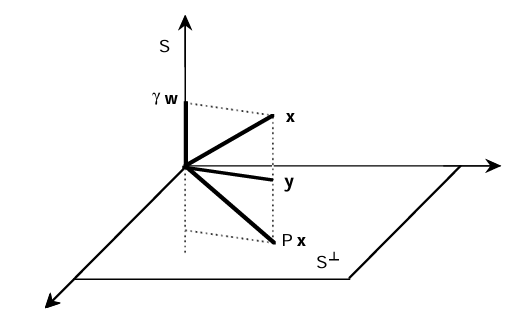
\includegraphics[width=0.8\textwidth]{Chapters/ch02/figure/riflessione_householder.png}
\caption{Riflessione del vettore \textbf{$x$} rispetto ad $S^{\perp}$}
\label{fig.:vect_riflesso}
\end{figure}
\end{itemize}


Come abbiamo visto, le matrici di Householder rappresentano una riflessione rispetto al piano ortogonale al vettore $\mathbf{v}$.
Quindi, dato un vettore $\mathbf{x}$, è sempre possibile costruire una matrice di Householder che riflette $\mathbf{x}$ in un vettore parallelo a $\mathbf{e}_1$
ed arrivare in modo intuitivo alla tesi del seguente teorema.

\begin{theorem}\label{teo:householder}
    Per ogni vettore $\textbf{x} \in \mathbb{R}^n$, con $\textbf{x} \neq 0$, si può identificare una \textcolor{orange}{matrice di Householder}
    tale che:
    \[
        \textcolor{orange}{P\mathbf{x} = \alpha \mathbf{e}_1 \quad \textcolor{black}{con} \quad \alpha \in \mathbb{R}}
    \]
    Dove \textcolor{orange}{$\alpha$} rappresenta una costante opportuna e:
    \[
    \textcolor{orange}{\textbf{v} = \mathbf{x} - \alpha \mathbf{e}_1, \quad \beta = \frac{2}{\|\mathbf{v}\|^2}}
    \]
\end{theorem}

\begin{proof}
    Vogliamo costruire esplicitamente $\mathbf{v}$ e $\beta$ tali che $P = I - \beta \mathbf{v}\mathbf{v}^t$ 
    soddisfi $P\mathbf{x} = \alpha \mathbf{e}_1$.

    \textbf{Passo 1: determinazione di $\alpha$.}
    Poiché $P$ è unitaria ($P^t P = I$), essa preserva la norma euclidea:
    \[
        \|\mathbf{x}\| = \|P\mathbf{x}\| = \|\alpha \mathbf{e}_1\| = |\alpha|.
    \]
    Quindi necessariamente $|\alpha| = \|\mathbf{x}\|$. Per evitare cancellazione numerica nella scelta di $\mathbf{v}$,
    si sceglie $\alpha$ con segno \textit{opposto} alla prima componente $x_1$ di $\mathbf{x}$:
    \[
        \alpha = -\,\mathrm{sgn}(x_1)\,\|\mathbf{x}\|, \qquad
        \text{con} \quad \mathrm{sgn}(x_1) = \begin{cases} \dfrac{x_1}{|x_1|} & \text{se } x_1 \neq 0 \\ 1 & \text{se } x_1 = 0. \end{cases}
    \]

    \textbf{Passo 2: scelta di $\mathbf{v}$.}
    La condizione $P\mathbf{x} = \alpha \mathbf{e}_1$ si riscrive come:
    \[
        (I - \beta \mathbf{v}\mathbf{v}^t)\mathbf{x} = \alpha \mathbf{e}_1
        \quad\Longrightarrow\quad
        \beta\,(\mathbf{v}^t \mathbf{x})\,\mathbf{v} = \mathbf{x} - \alpha \mathbf{e}_1.
    \]
    Questa equazione è soddisfatta scegliendo:
    \[
        \mathbf{v} = \mathbf{x} - \alpha \mathbf{e}_1.
    \]
    Notiamo che $\mathbf{v} \neq \mathbf{0}$: se fosse $\mathbf{v} = \mathbf{0}$, allora $\mathbf{x} = \alpha \mathbf{e}_1$
    con $\alpha = -\mathrm{sgn}(x_1)\|\mathbf{x}\|$, ma questo implicherebbe $x_1 = \alpha = -|x_1|$, cioè $|x_1| = 0$,
    contraddizione con $\mathbf{x} \neq \mathbf{0}$.

    \textbf{Passo 3: determinazione di $\beta$.}
    Con la scelta $\mathbf{v} = \mathbf{x} - \alpha \mathbf{e}_1$ si calcola:
    \[
        \mathbf{v}^t \mathbf{x} = (\mathbf{x} - \alpha \mathbf{e}_1)^t \mathbf{x}
        = \|\mathbf{x}\|^2 - \alpha x_1.
    \]
    Osserviamo inoltre che:
    \[
        \|\mathbf{v}\|^2 = \|\mathbf{x} - \alpha \mathbf{e}_1\|^2 = \|\mathbf{x}\|^2 - 2\alpha x_1 + \alpha^2
        = 2\|\mathbf{x}\|^2 - 2\alpha x_1 = 2(\mathbf{v}^t \mathbf{x}).
    \]
    Sostituendo nella condizione $\beta(\mathbf{v}^t\mathbf{x})\mathbf{v} = \mathbf{v}$:
    \[
        \beta\,(\mathbf{v}^t \mathbf{x}) = 1
        \quad\Longrightarrow\quad
        \beta = \frac{1}{\mathbf{v}^t \mathbf{x}} = \frac{2}{\|\mathbf{v}\|^2} = \frac{2}{\|\mathbf{x} - \alpha \mathbf{e}_1\|^2}.
    \]
    La matrice $P = I - \beta \mathbf{v}\mathbf{v}^t$ così costruita è quindi la Householder cercata.
\end{proof}

%=============================================================================================
%In questo capitolo si pongono le base per la fattorizzazione di una generica matrice quadrata
%=============================================================================================
\subsection{Fattorizzazione di matrici}

In questo paragrafo si introduce un teorema fondamentale per la fattorizzazione di matrici quadrate, che sarà alla base di molti metodi diretti per la risoluzione di sistemi lineari.

\begin{theorem}[Fattorizzazione di matrici quadrate]\label{teorema:fatt_matrici_quadrate}
    Si può sempre \textcolor{orange}{fattorizzare} una matrice $A \in \mathbb{R}^{n \times n}$ in un prodotto di due matrici $E$ ed $U$,
    dove $E$ è un prodotto di matrici elementari e $U$ è una matrice triangolare superiore:
    \[\textcolor{orange}{A = EU}\]
\end{theorem}

\begin{proof}{(per induzione su n)}

    Sia $A$ una matrice $n \times n$.
    Pensiamo ad $A$ come ad una matrice $A = A^{(1)}$ composta da una colonna $a_1$ e da una matrice $B$ composta dalle restanti colonne:
    \[A^{(1)} = [a_1 | B]\]
    Sia $E^{(1)}$ una matrice elementare non singolare che annulli le componenti di $a_1$ ad eccezione della prima, ovvero:
    \[E^{(1)} a_1 = a_{11} e_1\]
    Moltiplicando entrambi i lati per $E^{(1)}$, otteniamo:
    \[A^{(2)} = E^{(1)} A^{(1)} = [\mathbf{b_1}|E^{(1)} B]\]
    Dove:
    \[
    A^{(2)} = \begin{bmatrix}
    \alpha & \textbf{c}^t \\
    \textbf{0} & B^{(2)}
    \end{bmatrix}
    \]
    Iterando n-1 volte questo processo sulla sottmatrice $B^{(2)}$, otteniamo una successione
    di matrici $A^{(k)} \, k = 1, 2, \ldots, n$ tali che:
    \[A^{(k)} = \begin{bmatrix}
    C^{(k)} & D^{(k)} \\
    \mathbf{0} & B^{(k)}
    \end{bmatrix}\]
    Dove $C^{(k)} \in \mathbb{R}^{(k-1) \times (k-1)}, D^{(k)} \in \mathbb{R}^{(k-1) \times (n-k+1)}, B^{(k)} \in \mathbb{R}^{(n-k+1) \times (n-k+1)}$.
    Inoltre ipotizziamo che $C^{(k)}$ sia triangolare superiore e che $B^{(k)}$ sia invertibile.
    
    Prendiamo ora la matrice elementare $F^{(k)} \in \mathbb{R}^{(n-k+1) \times (n-k+1)}$ che annulli le componenti della prima colonna di $B^{(k)}$ ad 
    eccezione della prima, ovvero:
    \[
    F^{(k)} B^{(k)} = \begin{bmatrix}
    \beta & \mathbf{d}^t \\
    \mathbf{0} & B^{(k+1)}
    \end{bmatrix}
    \]
    Definiamo ora la matrice elementare (ne viene evitata la dimostrazione) $E^{(k)}$ come:
    \[
    E^{(k)} = \begin{bmatrix}
    I_{k-1} & \mathbf{0} \\
    \mathbf{0} & F^{(k)}
    \end{bmatrix}
    \]
    Moltiplicando $E^{(k)}$ per $A^{(k)}$, otteniamo:
    \[A^{(k+1)} = E^{(k)} A^{(k)} = \begin{bmatrix}
    C^{(k)} & D^{(k)} \\
    \mathbf{0} & F^{(k)} B^{(k)}
    \end{bmatrix} =
    \begin{bmatrix} C^{(k)} & D^{(k)} \\ \mathbf{0} & \begin{bmatrix}
    \beta & \textbf{d}^t \\
    \textbf{0} & B^{(k+1)}
    \end{bmatrix} \end{bmatrix} =
    \begin{bmatrix} C^{(k+1)} & D^{(k+1)} \\ \mathbf{0} & B^{(k+1)} \end{bmatrix}
    \]
    Dove $C^{(k+1)}$ è ancora triangolare superiore e $B^{(k+1)}$, per il \textit{teorema dei minori e del minimo}, è invertibile.
    All' $(n-1)$-esimo passo, otteniamo:
    \[A^{(n)} = \begin{bmatrix} C^{(n)} & \textbf{g} \\ \mathbf{0}^t &\gamma \end{bmatrix}\]
    Dove $C^{(n)}$ è triangolare superiore e $\gamma$ è un numero reale diverso da zero e quindi $A^{(n)}$
    è una matrice triangolare superiore.
    
    Dato che $E(k)$ è non singolare per ogni $k = 1, 2, \ldots, n-1$, si ha:
    \[
        A = E^{(1)^{-1}} E^{(2)^{-1}} \cdots E^{(n-1)^{-1}} A^{(n)} = E A^{(n)} = EU \quad con \, E \, \mathit{matrice\ elementare}
    \]
    Da cui la tesi.
\end{proof}

%===============================================================================
%In questa sezione vediamo alcuni metodi per la fattorizzazione LU.
%===============================================================================
\section{Metodo di eliminazione di Gauss - Fattorizzazione LU} 

\begin{defi}[Metodo (di eliminazione) di Gauss - Fattorizzazione LU]
   Viene detto \textcolor{orange}{metodo (di eliminazione) di Gauss} o \textcolor{orange}{fattorizzazione LU} il procedimento
   descritto nella dimostrazione del teorema (\ref{teorema:fatt_matrici_quadrate}) quando la matrice \textcolor{orange}{$E$} è un
   prodotto di \textcolor{orange}{matrici elementari di Gauss}, ovvero:
   \textcolor{orange}{\[
   E^{(k)} = \begin{bmatrix}
    I & \mathbf{0}\\
    \mathbf{0} & M^{(k)}
   \end{bmatrix} =
   \begin{bmatrix}
    1 & \\
    & \ddots \\
    & & 1 \\
    & & -m_{k+1,k} & 1 \\
    & & \vdots & & \ddots \\
    & & -m_{nk} & & & 1
   \end{bmatrix}
    \]}
    Dove $M^{(k)}$ è una matrice elementare di Gauss di ordine $n-k+1$ ($M^{(k)} \in \mathbb{R}^{(n-k+1) \times (n-k+1)}$).

    Da cui si trova (ricordando che la classe delle matrici elementari non singolari è chiusa rispetto all'operazione di inversione):
    \textcolor{orange}{\[
    L = E^{-1} \dots E^{(n-1)^{-1}} = \begin{bmatrix}
    1 & \\
    m_{21} & \ddots \\
    \vdots &  \ddots & 1\\
    \vdots & &  m_{k+1,k} & \ddots \\
    \vdots & &  \vdots & \ddots & \ddots\\
    m_{n1} & \dots &  m_{nk} & \dots & m_{(n-1)n} & 1
    \end{bmatrix}
    \]}
    dove \textcolor{orange}{\[
    m_{ik} = \frac{a_{ik}^{(k)}}{a_{kk}^{(k)}}
    \]}
    con $i = k+1, k+2, \ldots, n$ e $k = 1, 2, \ldots, n-1$.
\end{defi}

\begin{example}[Fattorizzazione LU di una matrice $4 \times 4$]
Consideriamo il sistema lineare $Ax = b$ con:
\[
A =
\begin{bmatrix}
-2 & 4 & -1 & -1 \\
4 & -9 & 0 & 5 \\
-4 & 5 & -5 & 5 \\
-8 & 8 & -23 & 20
\end{bmatrix}
\qquad
b =
\begin{bmatrix}
12 \\
-32 \\
3 \\
-13
\end{bmatrix}
\]
Applichiamo il metodo di Gauss per risolvere il sistema.

Si pone:
\[
A^{(1)} = A
\]
Si costruiscono le matrici elementari di Gauss $E^{(k)}$.

\bigskip

\textbf{Primo passo:}
\[
E^{(1)} =
\begin{bmatrix}
1 & 0 & 0 & 0 \\
2 & 1 & 0 & 0 \\
-2 & 0 & 1 & 0 \\
-4 & 0 & 0 & 1
\end{bmatrix}
\]
\[
A^{(2)} = E^{(1)} A^{(1)} =
\begin{bmatrix}
-2 & 4 & -1 & -1 \\
0 & -1 & -2 & 3 \\
0 & -3 & -3 & 7 \\
0 & -8 & -19 & 24
\end{bmatrix}
\]

\textbf{Secondo passo:}
\[
E^{(2)} =
\begin{bmatrix}
1 & 0 & 0 & 0 \\
0 & 1 & 0 & 0 \\
0 & -3 & 1 & 0 \\
0 & -8 & 0 & 1
\end{bmatrix}
\]
\[
A^{(3)} = E^{(2)} A^{(2)} =
\begin{bmatrix}
-2 & 4 & -1 & -1 \\
0 & -1 & -2 & 3 \\
0 & 0 & 3 & -2 \\
0 & 0 & -3 & 0
\end{bmatrix}
\]

\textbf{Terzo passo:}
\[
E^{(3)} =
\begin{bmatrix}
1 & 0 & 0 & 0 \\
0 & 1 & 0 & 0 \\
0 & 0 & 1 & 0 \\
0 & 0 & 1 & 1
\end{bmatrix}
\]
\[
U = A^{(4)} = E^{(3)} A^{(3)} =
\begin{bmatrix}
-2 & 4 & -1 & -1 \\
0 & -1 & -2 & 3 \\
0 & 0 & 3 & -2 \\
0 & 0 & 0 & -2
\end{bmatrix}
\]

Abbiamo quindi ottenuto la fattorizzazione $A = LU$ con:
\[
U =
\begin{bmatrix}
-2 & 4 & -1 & -1 \\
0 & -1 & -2 & 3 \\
0 & 0 & 3 & -2 \\
0 & 0 & 0 & -2
\end{bmatrix}
\]
\[
L =
\begin{bmatrix}
1 & 0 & 0 & 0 \\
-2 & 1 & 0 & 0 \\
2 & 3 & 1 & 0 \\
4 & 8 & -1 & 1
\end{bmatrix}
\]
Implementando ora la risoluzione dei sistemi lineari ausiliari $Ly = b$ e $Ux = y$, otteniamo:
\[y =
\begin{bmatrix}12 \\
-8 \\
-9 \\
-4
\end{bmatrix}
\qquad
x = \begin{bmatrix}-1 \\
-2 \\
-3 \\
2
\end{bmatrix}
\]
Dove, ricordando che $L$ ed $U$ sono rispettivamente una matrice triangolare inferiore ed una matrice triangolare superiore,
abbiamo utilizzato il metodo di sostituzione in avanti ($forward \, solve$) per risolvere $Ly = b$ e il metodo di sostituzione 
all'indietro ($backward \, solve$) per risolvere $Ux = y$.
\end{example}


Come si può intuire, non è sempre possibile fattorizzare una matrice $A$ in un prodotto $LU$ senza dover effettuare alcuna "modifica" alla matrice $A$ stessa.

Ad esempio, se la matrice $A$ ha un elemento nullo sulla diagonale principale, risulta evidente che sia impossibile annullare le componenti di una colonna utilizzando una matrice elementare di Gauss, in quanto si avrebbe una divisione per zero:
\[m_{ik} = \frac{a_{ik}^{(k)}}{a_{kk}^{(k)}}\]

%teorema di esistenza ed unicità della fattorizzazione LU
\begin{theorem}[esistenza ed unicità della fattorizzazione LU]
    \label{teorema:esistenza_unicità_LU}
    Sia $A \in \mathbb{R}^{n \times n}$ una matrice quadrata e siano \textcolor{orange}{$A^{(k)}$} le sue \textcolor{orange}{sottomatrici principali di testa} di ordine $k$.

    Se $A^{(k)}$ è \textcolor{orange}{invertibile} per ogni $k = 1, 2, \ldots, n-1$, allora esiste ed è unica la fattorizzazione $LU$ di $A$.
\end{theorem}

\subsection{Pivoting parziale e totale}

La condizione richiesta dal teorema~\ref{teorema:esistenza_unicità_LU} (tutti i minori principali invertibili) è \textbf{difficile da verificare a priori}, specialmente per matrici di grande dimensione.

Per questo motivo, nell'implementazione pratica del metodo di Gauss si utilizzano due tecniche dette:
\textcolor{orange}{pivoting parziale} e \textcolor{orange}{pivoting totale}.  
Queste strategie garantiscono sempre l'applicabilità della fattorizzazione, evitando divisioni per zero o per numeri troppo piccoli (che amplificano gli errori numerici).

Il concetto è semplice e intuitivo: se l'elemento \textcolor{orange}{$a_{kk}^{(k)}$} (pivot) è nullo o molto piccolo, non si può procedere con l'eliminazione.  
La soluzione naturale consiste nello \textcolor{orange}{scambiare righe} (e talvolta colonne) per portare un elemento sufficientemente grande in posizione pivot.

Vediamo ora in dettaglio come funzionano e in che modo si differenziano i due metodi.

\begin{defi}[Pivoting parziale e totale]
    \label{def:pivoting_parziale}
    \begin{itemize}
        \item \textcolor{orange}{\textbf{Pivoting parziale:}}
        
        consiste nell'effettuare una \textcolor{orange}{permutazione} delle righe di \textcolor{orange}{$A^{(k)}$}
        per portare l'elemento di massimo modulo della colonna $k$ in posizione \textcolor{orange}{$(k,k)$}.\\[0.5em]   
        \item \textcolor{orange}{\textbf{Pivoting totale:}}
        
        consiste nell'effettuare \textcolor{orange}{permutazioni} sia di righe che di colonne
        di ogni matrice \textcolor{orange}{$A^{(k)}$}, scegliendo il massimo assoluto nel blocco \textcolor{orange}{$i,j \geq k$}.
    \end{itemize}
    
    \textcolor{orange}{In simboli (pivoting parziale):}
    \[
    \textcolor{orange}{A^{(k)} = P_k^{(k)} A^{(k)}}
    \]
    dove \textcolor{orange}{$P_k^{(k)}$} è la matrice di permutazione che scambia le righe $k$ ed $\ell$:
    \[
    \textcolor{orange}{(P_{k,\ell})_{ij} =
    \begin{cases}
        1 & \text{se } i = j < k \text{ o } i = j > \ell \\
        1 & \text{se } (i,j) = (k,\ell) \text{ o } (i,j) = (\ell,k) \\
        0 & \text{altrimenti}
    \end{cases}}
    \]
    
    Alla fine si ottiene la fattorizzazione:
    \[
    \textcolor{orange}{\Pi A = LU} \quad con \textcolor{orange}{ \quad 
    \Pi = (P_{n-1}^{(n-1)} \cdots P_1^{(1)})^{-1}}
    \]
\end{defi}

\begin{obs}
    Il simbolo $=$ nella formula  $\textcolor{orange}{A^{(k)} = P_k^{(k)} A^{(k)}}$ è usato in senso "operativo", come nell'informatica.

    Dopo l'applicazione della permutazione $P^{(k)}$, la nuova matrice $A^{(k)}$ \textbf{sostituisce} quella precedente nei passi successivi dell'algoritmo.
\end{obs}
È evidente che il \textbf{pivoting totale}, dovendo cercare il massimo assoluto nell'intero blocco sottodiagonale, ha un \textbf{costo computazionale maggiore} rispetto al pivoting parziale.

Tuttavia, il pivoting totale offre una maggiore garanzia di stabilità numerica, controllando meglio la crescita degli elementi intermedi e riducendo l'amplificazione degli errori di arrotondamento.
\subsection{Fattorizzazione di Gauss Jordan}
Il \textcolor{orange}{metodo di Gauss-Jordan} costituisce una variante del \textcolor{orange}{metodo di Gauss} in cui, oltre all'eliminazione degli elementi \textbf{sotto} la diagonale principale,
si procede anche all'annullamento degli elementi \textbf{sopra} la diagonale principale.

Questo processo porta direttamente alla matrice \textbf{identità}, trasformando il sistema $Ax=b$ nella forma risolta $x = A^{-1}b$.

Alla fine si ottiene la fattorizzazione:
\[
\textcolor{orange}{A = LU} \quad con \textcolor{orange}{ \quad U = A^{(n)}}
\]
Dove \textcolor{orange}{$A^{(n)}$} è una matrice \textcolor{orange}{diagonale}.

\begin{obs}
Solitamente si evita di implementare il metodo di Gauss-Jordan perche'non offre una maggiore stabilità numerica rispetto al metodo di Gauss
(oltre ad avere un costo computazionale elevato).
\end{obs}

\section{Metodo di  Householder - Fattorizzazione QR}

Come si può intuire, per analogia con il metodo di Gauss, è possibile utilizzare le matrici elementari di Householder per fattorizzare una matrice $A \in \mathbb{R}^{m \times n}$ in un prodotto $QR$, grazie ai teoremi (\ref{teorema:fatt_matrici_quadrate}) e (\ref{teo:householder}).

\begin{defi}[Metodo di Householder - Fattorizzazione QR]
    Viene detto \textcolor{orange}{metodo di Householder} o \textcolor{orange}{fattorizzazione QR} il procedimento
    descritto nella dimostrazione del teorema (\ref{teorema:fatt_matrici_quadrate}) quando la matrice \textcolor{orange}{$E$} è un
    prodotto di \textcolor{orange}{matrici elementari di Householder}, dove
    \textcolor{orange}{\[
    E^{(k)} =
    \begin{bmatrix}
        I_{k-1} & \mathbf{0}\\
        \mathbf{0} & P^{(k)}
    \end{bmatrix} =
    \begin{bmatrix}
        1 & \\
        & \ddots \\
        & & 1 \\
        & & & P^{(k)}
    \end{bmatrix}
    \]}
    e $\textcolor{orange}{P^{(k)}}$ è la \textcolor{orange}{matrice di Householder} di ordine $n-k+1$ che azzera le componenti
    sotto la diagonale nella $k$-esima colonna di $A^{(k)}$.\\

    \textbf{Costruzione esplicita di $P^{(k)}$.}
    La matreice \textcolor{orange}{$P^{(k)}$} è costruita seguendo il procedimento descritto nel teorema (\ref{teo:householder}), ovvero:
    \[\textcolor{orange}{P^{(k)} = I - \beta \mathbf{v} \mathbf{v}^t}\]
    con:
    \[\textcolor{orange}{\mathbf{v} = \mathbf{x} - \alpha \mathbf{e}_1, \quad \beta = \frac{2}{\|\mathbf{v}\|^2}}\]
    dove $\mathbf{x}$ è la $k$-esima colonna di $A^{(k)}$ a partire dalla riga $k$-esima, $\mathbf{e}_1$ è il primo vettore della base canonica di $\mathbb{R}^{n-k+1}$ e $\alpha$ è scelto come:
    \[\textcolor{orange}{\alpha = -\,\mathrm{sgn}(x_1)\,\|\mathbf{x}\|}\]

    Dato che, per un teorema di algebra lineare, $(AB)^t = B^t A^t$ e dato che \textcolor{orange}{$P^{(k)}$} è una matrice \textcolor{orange}{unitaria} ($P^{(k)^{-1}} = P^{(k)^t}$), si ha che:
    \[\textcolor{orange}{Q = E^{(1)^{-1}} E^{(2){-1}} \cdots E^{(n-1)^{-1}} = E^{(1)^t} E^{(2)^t} \cdots E^{(n-1)^t} = (E^{(n-1)}E^{(n-2)} \cdots E^{(1)})^t}\]
    è una matrice \textcolor{orange}{unitaria} e che:
    \[\textcolor{orange}{R = A^{(n)} = E^{(n-1)} \cdots E^{(2)} E^{(1)} A}\]
    è una matrice \textcolor{orange}{triangolare superiore}.
\end{defi}

\begin{example}[Esempio di fattorizzazione QR di una matrice $3 \times 3$]
Consideriamo la matrice:
\[
A=
\begin{bmatrix}
2 & 1 & 1\\
0 & 3 & 1\\
0 & 4 & 1
\end{bmatrix}
\]
e applichiamo il procedimento della definizione:
\[
A^{(1)}=A, \qquad A^{(k+1)} = E^{(k)}A^{(k)}
\]

\textbf{Passo $k=1$.} Si considera la prima colonna di $A^{(1)}$ a partire dalla riga 1:
\[
\mathbf{x}^{(1)} =
\begin{bmatrix}
2\\
0\\
0
\end{bmatrix},
\qquad
\alpha_1 = -\mathrm{sgn}(2)\,\|\mathbf{x}^{(1)}\|=-2
\]
\[
\mathbf{v}^{(1)} = \mathbf{x}^{(1)}-\alpha_1\mathbf{e}_1=
\begin{bmatrix}
4\\
0\\
0
\end{bmatrix},
\qquad
\beta_1=\frac{2}{\|\mathbf{v}^{(1)}\|^2}=\frac{1}{8}
\]
\[
P^{(1)}=I-\beta_1\mathbf{v}^{(1)}\mathbf{v}^{(1)t}=
\begin{bmatrix}
-1 & 0 & 0\\
0 & 1 & 0\\
0 & 0 & 1
\end{bmatrix}
\]
Per $k=1$ vale $E^{(1)}=P^{(1)}$, quindi:
\[
A^{(2)}=E^{(1)}A^{(1)}=
\begin{bmatrix}
-2 & -1 & -1\\
0 & 3 & 1\\
0 & 4 & 1
\end{bmatrix}
\]

\textbf{Passo $k=2$.} Si lavora sulla seconda colonna di $A^{(2)}$ dalla riga 2 in poi:
\[
\mathbf{x}^{(2)}=
\begin{bmatrix}
3\\
4
\end{bmatrix},
\qquad
\alpha_2=-\mathrm{sgn}(3)\,\|\mathbf{x}^{(2)}\|=-5
\]
\[
\mathbf{v}^{(2)}=\mathbf{x}^{(2)}-\alpha_2\mathbf{e}_1=
\begin{bmatrix}
8\\
4
\end{bmatrix},
\qquad
\beta_2=\frac{2}{\|\mathbf{v}^{(2)}\|^2}=\frac{1}{40}
\]
\[
P^{(2)}=I-\beta_2\mathbf{v}^{(2)}\mathbf{v}^{(2)t}=
\begin{bmatrix}
-\frac{3}{5} & -\frac{4}{5}\\
-\frac{4}{5} & \frac{3}{5}
\end{bmatrix}
\]
L'estensione a ordine 3 è:
\[
E^{(2)}=
\begin{bmatrix}
1 & 0 & 0\\
0 & -\frac{3}{5} & -\frac{4}{5}\\
0 & -\frac{4}{5} & \frac{3}{5}
\end{bmatrix}
\]
\[
R=A^{(3)}=E^{(2)}A^{(2)}=
\begin{bmatrix}
-2 & -1 & -1\\
0 & -5 & -\frac{7}{5}\\
0 & 0 & -\frac{1}{5}
\end{bmatrix}
\]

Infine, dalla definizione:
\[
Q=
\begin{bmatrix}
 -1 & 0 & 0\\
 0 & -\frac{3}{5} & -\frac{4}{5}\\
 0 & -\frac{4}{5} & \frac{3}{5}
\end{bmatrix}
\]
con:
\[
Q={(E^{(2)}E^{(1)})}^t
\]
e si verifica immediatamente che $Q^{t}Q=I$ e $A=QR$.
\end{example}


